\documentclass[10pt,letterpaper]{article}
%\usepackage{fullpage}
\usepackage[latin1]{inputenc}
\usepackage{amsmath}
\usepackage{amsfonts}
\usepackage{amssymb}
\usepackage{graphicx}
\author{S. Zain Hoda and Rui Xiong Kee}
\title{Implementation of a Mortgage Backed Security (MBS) Pricing Model}
\begin{document}
\maketitle
\begin{center}
ORF 535: Computational Finance in C++\\
Prof. Ren\'e Carmona\\
Princeton University\\
Bendheim Center for Finance
\end{center}
\section*{Abstract}
We implement a Mortgage Backed Security (MBS) pricing tool. The model employs a Hull-White single-factor short rate model calibrated to the swaption volatility matrix. Mortgage rates are determined using a regression on 10 year treasury yields, using both the original and first-differenced time series as a check against spurious regression. Our pricing tool finds the price of an MBS given the OAS or vice versa. Additionally, given the price it can find the Zero Volatility (ZV) spread. It also determines duration and convexity for hedging purposes. Regular (non-callable) bonds exhibit a linear relationship between coupon rate and price. Mortgage Backed Securities exhibit a negative convexity due the ability of borrowers to prepay. Our pricing tool exhibits the basic property of negative convexity.\footnote{\begin{normalsize}Please note that this document is not as long as it appears; for readability we used large margins and we have many figures embedded into the document. The \LaTeX{} code we used to produce this document is slightly over 8 pages.\end{normalsize}}
\newpage
\section{Introduction}
Mortgage Pass-Through Securities, more commonly known as Mortgage Backed Securities, are bonds that are backed by a pool of mortgages. They are extremely liquid and are a very important part of the market, and were in the spotlight recently due to the flurry of recent market activity concerning subprime mortgages. The most important differentiating factor of an MBS and a regular bond is that of prepayment.\\
\\
In the discussion of the math, we also provide a reference to respective segment of the program that implements the math-finance topic discussed in a particular section.
\section{Components of the Model}
\subsection{Interest Rate Model}
\begin{verbatim}
Class: SimulatedTermStructure
\end{verbatim}
We take as an input today's instantaneous forward curve. To achieve this we took eight points on the LIBOR swap curve as the yield curve and fit a smoothed spline through those points. Points on the instantaneous forward curve are then given by:
\begin{eqnarray}
f(t,T) & = & \dfrac{\partial}{\partial T} y(t,T)(T - t) + y(t,T)
\end{eqnarray}
Given today's forward curve we produce simulations of the interest rate over the time period of the mortgages we are attempting to price. A somewhat simple way to do this is to use Hull-White's Extended Vasicek model so that we can fit the current forward curve perfectly.
We used the following form of the Extended Vasicek.
\begin{eqnarray}
dr_t & = & a (\bar{r_t} - r_t)dt + \sigma dW_t\\
\bar{r_t} & = & f(t_0, t) + \dfrac{1}{a} \dfrac{\partial f(t_0,t)}{\partial t} + \dfrac{\sigma^2}{2a^2} \left( 1 - e^{-2a(t-t_0)} \right) 
\end{eqnarray}
It remains to choose parameters $a$ and $\sigma$. In an ideal setting, we can find $a$ and $\sigma$ by calibrating our model to the market ATM swaption volatility matrix. We have as input the market implied swaption volatilites. Black's swaption pricing formula then gives us the swaption prices:
\begin{eqnarray}
PS^{Black}(0) & = & [S_n(0) N(d_1) - K N(d_2)] \sum_{i=1}^n p(0, T_i) \tau_i \\
d_1 & = & \dfrac{\log(\frac{S_n(0)}{K}) + \sigma_{imp}^2 T_0}{\sigma_{imp} \sqrt{T_0}}\\
d_2 & = & d_1 - \sigma_{imp} \sqrt{T_0}
\end{eqnarray}
On the other hand, we can arrive at an estimated swaption price using Monte Carlo estimation of the expectation, under the risk-neutral measure, of the discounted payoff of the swaption:
\begin{eqnarray}
E_t^Q[e^{-\int_t^{T_0} r_s ds} (S_n(T_0) - K)^{+} \sum_{i=1}^n \tau_i P(T_0, T_i)]
\end{eqnarray}
$\tau_i$ is $T_i - T_{i-1}$; $T_i$ are the LIBOR fixing dates, where $P(t,T)$ is the price of a zero coupon bond starting at $t$ and maturing at $T$. The swap rate $S_n(t)$ is given by:
\begin{eqnarray}
R_{swap}(t,T) & = & \dfrac{1 - P(t,T_N)}{\sum_{j=1}^N P(t,T_j)\tau_j }\\
P(t,T) & = & e^{-A(t,T) - B(t,T) r_t}\\
B(t,T) & = & \dfrac{1-e^{-a(T-t)}}{a}\\
A(t,T) & = & - \dfrac{\sigma^2}{2} \int_t^T B^2(s,T)ds + \int_t^T a \bar{r_t} B(s,T) ds
\end{eqnarray}
Calibration then is the process of finding $a$ and $\sigma$ to minimize the squared difference between the market swaption prices and the Monte Carlo estimated prices:
\begin{eqnarray}
\min_{a,\sigma} \: [\text{Swaption}_{mkt} - \text{Swaption}_{MC}]^2
\end{eqnarray}
In practice we are faced with two constraints.  The first is that we only have two time-homogeneous parameters, a and sigma, with which to potentially match many swaption prices.  The second is that using our small scale implementation to calibrate to several points may be computationally prohibitive.  As such, we decided to match one point of the volatility matrix, which we choose to be the 5yr5yr ATM\footnote{5 year swap rate starting 5 years from today} swaption volatility. \\
\\
We employ a 2-step procedure to calibrate our model to the 5yr5yr swaption volatility under our scaled-down approach.  In the first step, we use historical data to estimate ``reasonable" values for $a$ and $\sigma$.  In order to do this, we consider the regular Vasicek model:
\begin{eqnarray}
dr_t = a(\bar{r} - r_t)dt + \sigma dW_t
\end{eqnarray}
Which we can rewrite as an AR(1):
\begin{eqnarray}
r_t = (1 - \rho)\alpha + \rho r_{t-1} + \epsilon_t,
\end{eqnarray}
where $\epsilon_t \sim N(0, \sigma^2_\Delta)$ with $\sigma^2_\Delta = \sigma^2(1 - \exp(-2\kappa \Delta))/(2 \Delta)$, $\rho = \exp(-\kappa \Delta)$.  Where $\Delta$ is 1/frequency of data.  Using 3 month T-bill rates as a proxy for the short rate, and considering weekly data ($\Delta$ = 1/52) from the Federal Reserve Board from 1982 - 2004, we find the following estimates \footnote{see appendix for S-plus code}:\\
$\sigma: 0.01219293$\\
$a: 0.1686036$\\
With these values in mind, we fix the value of $a$, varying only the $\sigma$ parameter in order to match the Monte Carlo price to the market swaption price.\\
\begin{center}
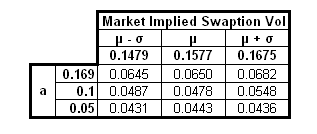
\includegraphics[scale=0.7]{mktvoltable.png}\\
$\mu$ = Mean of market implied swaption volatility (5/2006 - 5/2007)\\
$\sigma$ = SD of market implied swaption volatility (5/2006 - 5/2007)\\
\end{center}
From the table above, we see that the choice of $a = 0.1$ strikes a good balance between keeping $a$ relatively close to its historical value, while simultaneously ensuring that the $\sigma$ we get from calibration is close to historical sigma.\\
\begin{center}
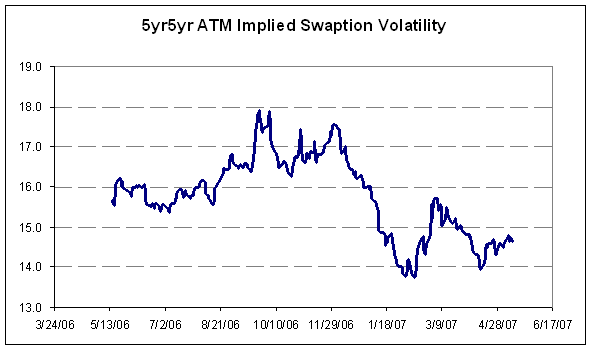
\includegraphics[scale=0.5]{swaption.png}\\
Mean = 15.77, Standard Deviation = 0.9841
\end{center}
\subsection{Mortgage Rate Model}
\begin{verbatim}
Class: MortgageRateGenerator
\end{verbatim}
Since mortgage rates are highly correlated to swap rates, one method for simulating mortgage rates is to take simulated 10-year swap rates and regress these with the historical mortgage rates. Ordinarily, one would compute the future swap rates. However, we chose to get the 10-year yield curve from the short rates to save on computation time. We performed a regression of historical 30-year fixed mortgage rates against 10-year treasury yields over the period 1994 to 2003.
\begin{verbatim}
Residual Standard Error = 0.0024,  Multiple R-Square = 0.9179
N = 2501,  F-statistic = 27947.97 on 1 and 2499 df, p-value = 0

numeric matrix: 2 rows, 4 columns. 
            coef std.err   t.stat p.value 
Intercept 0.0289  0.0003 106.7269       0
        X 0.7813  0.0047 167.1765       0
\end{verbatim}
There is always the worry that these are two nonstationary time series. To be more rigorous, we check to see if they are cointegrated variables whose first differences are stationary. This check involves performing a unit root test on the regression residuals. Based on the Augmented Dickey-Fuller test we reject, at the 5\% critical level, the null hypothesis of a unit root with a p-value of 0.02744 and thus find evidence in favor of cointegration.\\
\\
Another way to avoid the problem of nonstationary variables is to do a regression of their first differences instead.
\begin{verbatim}
Residual Standard Error = 0.0001,  Multiple R-Square = 0.0367
N = 2500,  F-statistic = 95.0948 on 1 and 2498 df, p-value = 0

            coef std.err  t.stat p.value 
Intercept 0.0000  0.0000 -2.3217  0.0203
        X 0.0346  0.0035  9.7517  0.0000
\end{verbatim}
We see that the relationship between the first order difference is also significant. We can check how well the coefficients of the regression and the first difference regression are able to predict the mortgage rates. Using the formulas $\hat{Y}_{t+1} - Y_{t} = 0 + 0.346 (X_{t+1}-X_{t})$ and $\hat{Y}_{t+1} = 0.0289 + 0.7813X_{t+1}$ we find that our predicted $\hat{Y}_t+1$ are similar (see graph). As such we conclude that using the regression coefficients of mortgage rate on 10 year treasury yield is valid. \\
\begin{center}
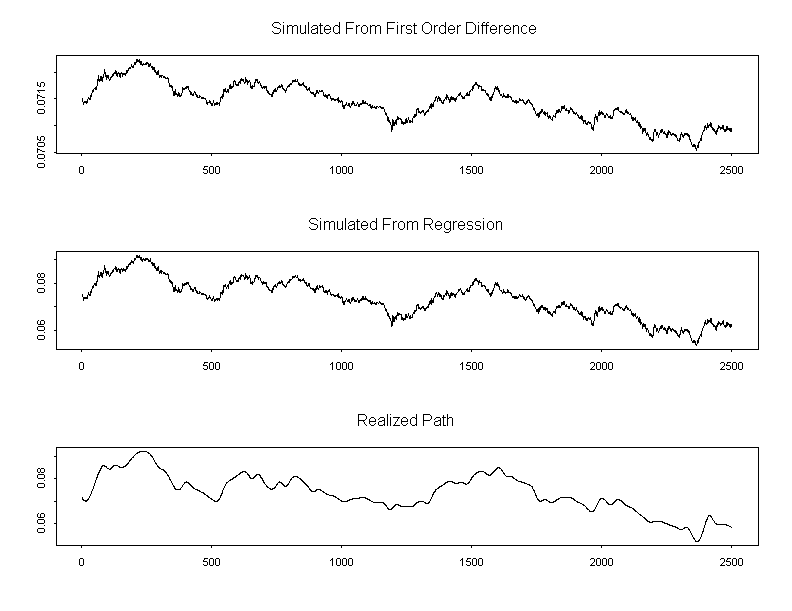
\includegraphics[scale=0.45]{regressionprediction.png}\\
\end{center}
We have provided a C++ implementation of ordinary least squares regression.
\subsection{Prepayment Model}
\begin{verbatim}
Class: cprPathGenerator
\end{verbatim}
Given the mortgage rate, we want to consider when the borrowers will prepay their loans. We have provided two implementations of a prepayment model (called A and B in the program). Prepayment model A is modeled after slides presented by John Naud whereas prepayment model B is taken from a Fannie Mae paper (Chen 2004) to use as a check. Many factors contribute to when the prepayments occur. For simplicity we choose a few of these factors and attempt to model them. \\
Model A uses the following formula to generate CPR (Constant Prepayment Rate - the annualized rate of prepayment at each time):
\begin{eqnarray}
CPR(t) = RI(t)BM(t) + AGE(t)MM(t)
\end{eqnarray}
while Model B uses:
\begin{eqnarray}
CPR(t) & = & RI(t) AGE(t) MM(t) BM(t)
\end{eqnarray}
Where $RI(t)$ is the refinancing incentive, $BM(t)$ refers to burnout, $AGE(t)$ is the seasoning ramp, and $MM(t)$ is the monthly multiplier. Each of these factors of CPR are explained in individual sections to follow.
\subsubsection{Refinancing Incentive}
Mortgage borrowers have the option to prepay their loans and take out a new loan with a lower mortgage rate. If borrowers exercised this option optimally, we would see that anytime the current mortgage rate falls below the mortgage rate of the borrower, they would refinance (assuming no transaction costs).
\begin{center}
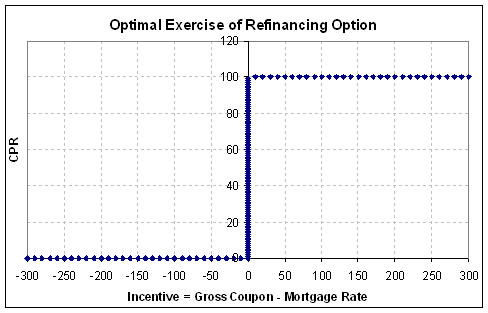
\includegraphics[scale=0.5]{optimalexercise.png}\\
\end{center}
Empirically borrowers do not optimally excercise this option, resulting in an S-curve.
\begin{center}
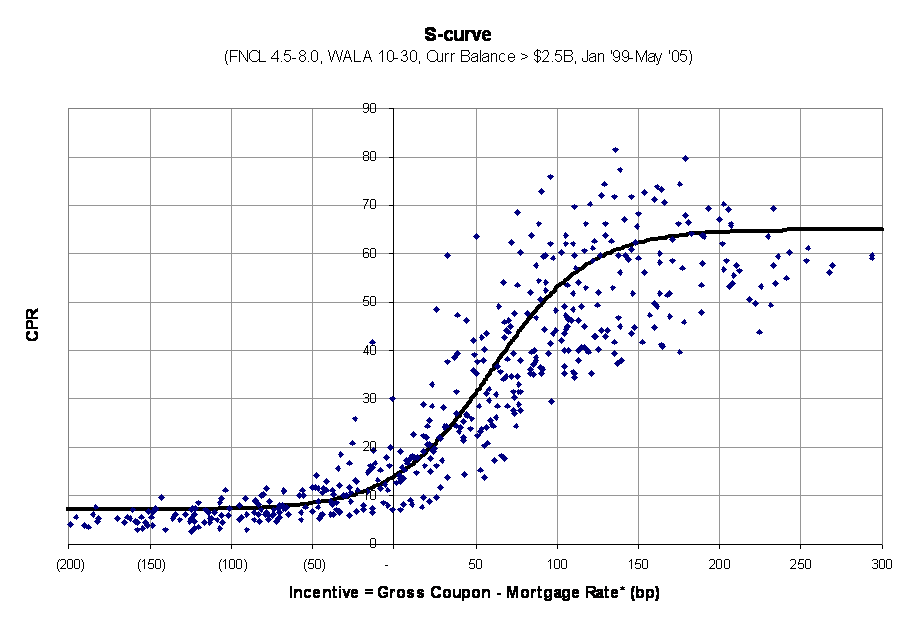
\includegraphics[scale=0.3]{suboptimalexercise.png}\\
(Courtesy Naud 2007)
\end{center}
For prepayment model A, we start by observing that the S-curve graph of CPR to incentive can be replicated by a normal cumulative distribution function (CDF), suitably shifted and rescaled. Our refinancing function thus employs the normal CDF:
\begin{eqnarray}
RI(t) & = & \Phi((\text{incentive} - \text{shift})\text{rescale})
\end{eqnarray}
Using appropriate values for shift and rescale.\\
Such an approach not only ensures the replication of empirically observed behavior, it also has theoretical underpinnings.  For instance, Kariya and Kobayashi (2000) suggest a model for the exit time of the $k$th mortgagor as:
\begin{eqnarray}
\tau_k = \min \lbrace j : WAC - R_j \geq c_j(k) \rbrace
\end{eqnarray}
Where $c_j(k)$ denotes the ``incentive threshold" of the $k$th mortgagor at time $j$, $WAC$ refers to the weighted average coupon at the time of the mortgage pool's issue (i.e. the mortgage rate we start with), and $R_j$ refers to the mortgage rate prevailing at time $j$. Note that if all mortgagors were optimal exercisers of their option to refinance, $c_j(k)$ should be 0. In the simplest model with no information on the $k$th mortgagor is available, Kariya and Kobayashi suggest that we can explain the heterogeneous response of mortgagors to refinancing incentive by having incentive thresholds $c_j(k)$ that are normally distributed in the mortgage pool. This is equivalent to having the refinancing CPR function in the form of a normal CDF.\\
\\
Model A uses the cumulative distribution function for a Gaussian random variable to produce the so-called ``S-curve" plus a seasoning ramp, whereas Model B uses the following formula:
\begin{eqnarray}
RI(t) & = & 0.28 + 0.14 \tan^{-1} \left( -8.571 + 430 (WAC - {r_{10,t-1}}) \right)
\end{eqnarray}
\begin{center}
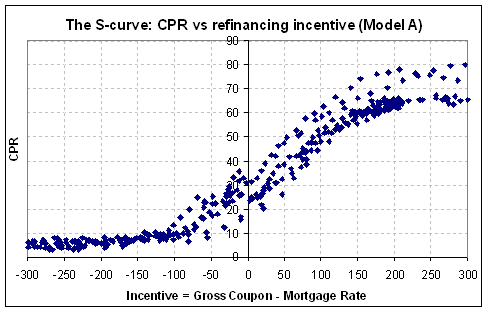
\includegraphics[scale=0.6]{CPRtoRefinChartModelA.png}\\
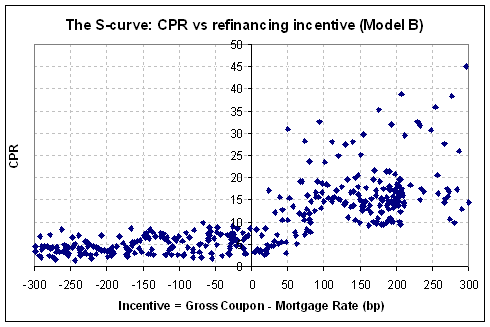
\includegraphics[scale=0.6]{CPRtoRefinChartModelB.png}\\
\end{center}
\subsubsection{Seasoning Ramp}
People do not tend to move (and hence prepay) within the first few months of buying a new house. The prepayment rate increases as the loan age increases up to a certain point.
\begin{quote}
The PSA model is one of several models used to calculate and manage prepayment risk. The PSA model acknowledges that prepayment assumptions will change during the life of the obligation and affect the yield of the security. The model assumes a gradual rise in prepayments, which peaks after 30 months. The standard increase amount is 0.2\%, so an indicator of 100\% implies that the rate will increase monthly by 0.2\% (the standard increase), whereas an indicator of 0\% implies no monthly changes of the prepayment rate.\footnote{http://www.investopedia.com/terms/p/psa.asp} 
\end{quote}
\begin{eqnarray}
AGE(t) & = & \min \left( 1, \dfrac{t}{30} \right)
\end{eqnarray}
\begin{center}
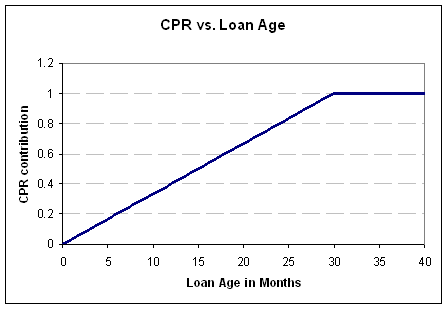
\includegraphics[scale=0.6]{seasoning.png}
\end{center}
\subsubsection{Monthly Multiplier}
$ MM(t) $ is $[0.7, 0.65, 0.85, 0.95, 1.0, 1.2, 1.1, 1.35, 1.15, 1.1, 1.0, 0.95]$ respective to the month due to the fact that turnover in the housing market varies by month.\footnote{Andrew Davidson \& Co Research Report}
\begin{center}
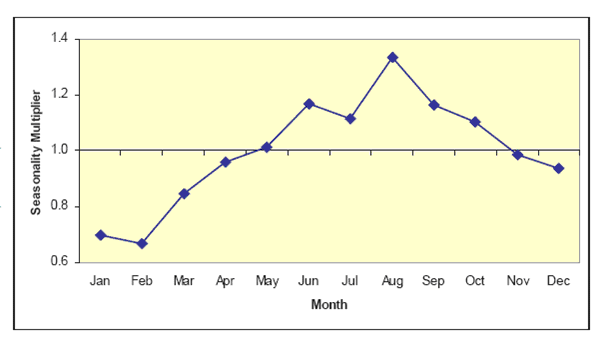
\includegraphics[scale=0.4]{monthlymultiplier.png}\\
\end{center}
\subsubsection{Burnout Multiplier}
Burnout refers to the empirical slowdown of prepayments due to mortgage-rate changes following periods of intensive refinancings. The people who are most likely to respond to incentives to refinance do so early, leaving the pool with borrowers who are less likely to refinance. \footnote{Kalotay Yang Fabozzi 2004} 
\begin{eqnarray}
BM(t) & = & 0.3 + 0.7 \dfrac{\hat{B_{t-1}}}{\hat{B_0}}
\end{eqnarray}
Where $\hat{B_n}$ is defined in equation $\ref{burnoutb}$
\subsubsection{Other Approaches to Modeling Prepayment}
Kalotay, Yang and Fabozzi (KYF) treat the mortgagor's right to refinance as an American call option on mortgage rate with the weighted average coupon as its strike.  At each time, the mortgagor compares the value of exercise to the value of waiting.  In order to account for sub-optimal exercise of the option, KYF create a distribution of strike rates across the population of mortgagors. In other words, mortgagors who are slow to refinance (i.e. wait till the option is well into the money before exercising) do so because they believe that the strike is higher than it actually is, while mortgagors who refinance too soon believe that the strike is lower than it is.\\
\\
A much more basic attempt to model refinancing behavior is described in London (2005).  Here, refinancing CPR is fixed between certain bounds:\\
\begin{equation}
\label{londonrefinancing}
RI(j) = 
\begin{cases} 
0 & \text{if $R_0 - R_j > k_4$}\\
b_4 & \text{if $k_3 < R_0 - R_j \leq k_4$}\\
b_3 & \text{if $k_2 < R_0 - R_j \leq k_3$}\\
b_2 & \text{if $k_1 < R_0 - R_j \leq k_2$}\\
b_1 & \text{if $k_0 < R_0 - R_j \leq k_1$}\\
1 & \text{if $R_0 - R_j \leq k_0$}\\
\end{cases} 
\end{equation}
Where $k_4 > k_3 > k_2 > k_1 > k_0$ and $0 < b_4 < b_3 < b_2 < b_1 < b_0 < 1$ are positive constants. $R_0$ and $R_j$ have the same meaning as in equation $\ref{londonrefinancing}$.  In this approach, we are simply using a step function to approximate the S-curve of CPR against incentive.\\
\begin{center}
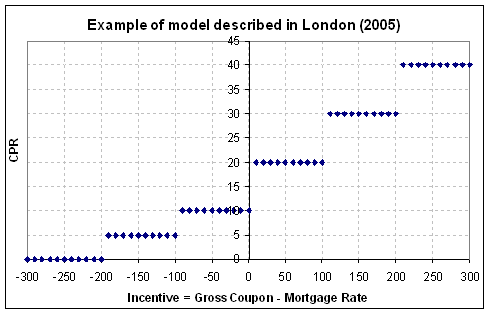
\includegraphics[scale=0.7]{londonmodel.png}\\
\end{center}
The method described in London's book is too simplistic for our purposes. However, there is a strong desire within academia to employ an options framework to analyze refinancing behavior, and in this respect, the methodology suggested by Kalotay, Yang and Fabozzi is appealing. However, we believe that our approach circumvents the modeling complexity of American options, while retaining the spirit of the approach - using a distribution of incentive thresholds to explain the suboptimal option exercise behavior of mortgagors. 
\subsection{Cashflow Model}
\begin{verbatim}
Class: CFgenerator
\end{verbatim}
Below is a table of several CPR scenatios and their cashflows. As a sanity check, we note that our cashflow generator matches the output in Naud (2007).\\
\begin{center}
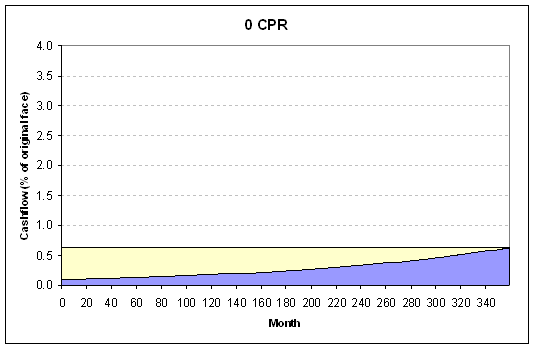
\includegraphics[scale=0.3]{0CPRchart.png}
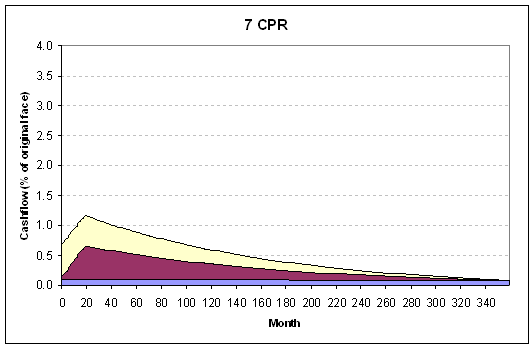
\includegraphics[scale=0.3]{7CPRchart.png}\\
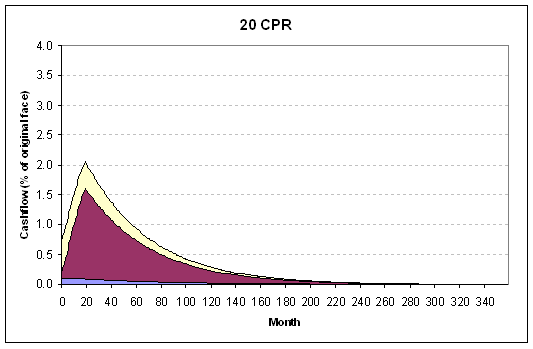
\includegraphics[scale=0.3]{20CPRchart.png}
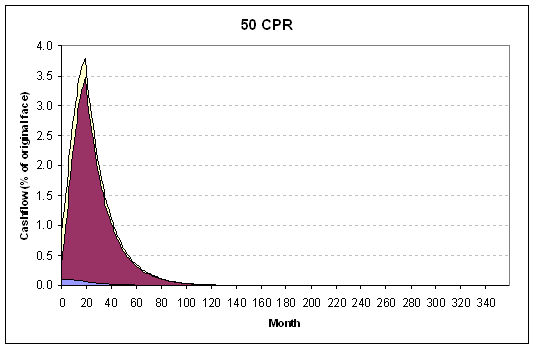
\includegraphics[scale=0.3]{50CPRchart.png}\\
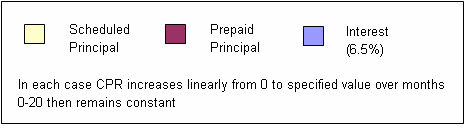
\includegraphics[scale=0.4]{legendCPR.png}\\
\end{center}
The cashflow model is just a straightforward implementation of the formulas below.\\
\textbf{Zero Prepayments:}
\begin{eqnarray}
CF_n & = & SP_n + I_n\\
SP_n & = & g \dfrac{d^{N-n+1}}{1-d^N}\\
I_n & = & c \dfrac{1 - d^{N-n+1}}{1-d^N}\\
B_n & = & \dfrac{1-d^{N-n}}{1-d^N}
\end{eqnarray}
\textbf{Nonzero Prepayments:}
\begin{eqnarray}
\hat{CF_n} & = & \hat{SP_n} + \hat{PP_n} + \hat{I_n}\\
\hat{SP_n} & = & Q_{n-1} SP_n\\
\hat{PP_n} & = & (\hat{B_{n-1}} - \hat{SP_n})SMM_n\\
\hat{I_n} & = & Q_{n-1}I_n\\
\label{burnoutb} \hat{B_n} & = & \hat{B_{n-1}} - \hat{SP_n} - \hat{PP_n} = Q_n B_n
\end{eqnarray}
Where $g$ is the gross monthly coupon on underlying loans; $c$ is the net monthly coupon received by MBS holder, $N$ is the original loan maturity in months; $n$ is the loan age in months; $B_n$ is the remaining principal balance per unit of original balance after $n^{th}$ monthly payment assuming zero prepayments; $ d = 1/(1 + g)$; $ (1 - SMM) = (1 - CPR)^{1/12}$; $F_n$ is the pool factor (actual remaining balance per dollar of original principal); $Q_n = F_n / B_n$ is the fraction of the pool that has not yet prepaid; $Q_n = Q_{n-1} (1 - SMM)$, $Q_0 = 1$.\\
\section{Combining the Components}
\begin{verbatim}Class: MBS \end{verbatim}
This class starts the chain of computations and simulations given the necessary input parameters to the model.
\subsection{Computing the Option Adjusted Spread or Price}
\begin{verbatim}Method: MBS->OAspread 
        MBS->getPrice \end{verbatim}
Given cashflows $CF_j$, asset pricing would tell us that we would just have to discount these cash flows under the risk neutral measure to produce the price.
\begin{eqnarray}
p_t & = & E_t^Q \left[ \sum_{j=1}^N e^{-\int_t^{t_j} r_s ds }CF_j \right] \\
& = & E_t^Q \left[ \sum_{j=1}^N e^{-\int_t^{t_j} f(s,s) ds }CF_j \right]
\end{eqnarray}
However, we could only do this if we knew when people prepayed. Unfortunately prepayment is not determinstic nor is it excercised optimally so we have to simulate this as well and there will be a certain error in the price. To account for this error, we add the Option Adjusted Spread.
\begin{eqnarray}
p_t(\lambda) & = & E_t^Q \left[ \sum_{j=1}^N e^{-\int_t^{t_j} f(s,s) ds - \lambda (t_j - t)}CF_j \right]
\end{eqnarray}
Given either the price or the OAS, using this formula we can compute the other value. 
\subsubsection{Computing the Zero Volatility Spread}
\begin{verbatim}Method: MBS->ZVspread \end{verbatim}
We built the apparatus to compute the OAS, which is a more difficult problem. To compute the ZV spread, we go through the same process as for OAS except instead of using simulated interest rates we use today's deterministic forward rates and use $\lambda_0$ instead of $\lambda$.
\begin{eqnarray}
p_t(\lambda) & = & \sum_{j=1}^N e^{-\int_t^{t_j} f(t,s) ds - \lambda_0 (t_j - t)}CF_j
\end{eqnarray}
\subsection{Comparing Our Spreads with Bloomberg}
We compare our ZV spread and our OAS with Bloomberg. For both, we have spread values that are around the same order as Bloomberg. Our ZV spread more closely matches Bloomberg values because only the cashflows are predicted; the discount rates used are today's forward curve.
\begin{center}
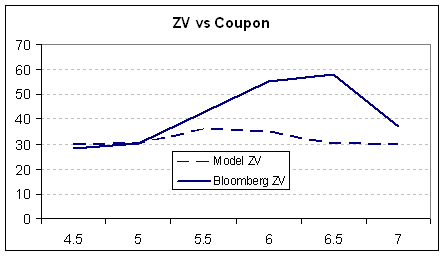
\includegraphics[scale=0.5]{zvvscpn.png}
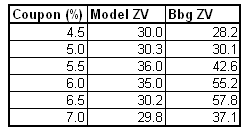
\includegraphics[scale=0.5]{zvvscpntable.png}\\
\end{center}
We would expect the OAS to diverge more from Bloomberg because of the added prediction of interest rates, which is again what we see.
\begin{center}
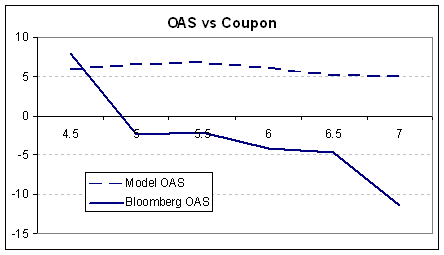
\includegraphics[scale=0.5]{oasvscpn.png}
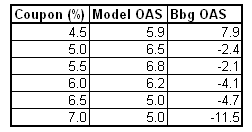
\includegraphics[scale=0.5]{oasvscpntable.png}\\
\end{center}
\subsection{Duration and Convexity}
\begin{verbatim}Method: MBS->OAduration 
        MBS->OAconvexity \end{verbatim}
The mathematically correct method to compute duration and convexity is to compute the first and second derivatives. However, a common numerical alternative is effective duration and effective convexity. We use $\Delta \lambda$ of 50 basis points.
\begin{eqnarray}
D_{eff} & = & \dfrac{P(\lambda - \Delta \lambda) - P(\lambda + \Delta \lambda)}{2P(\lambda)\Delta \lambda}\\
C_{eff} & = & \dfrac{P(\lambda + \Delta \lambda) + P(\lambda - \Delta \lambda) - 2P(\lambda)}{P(\lambda)(\Delta \lambda)^2}
\end{eqnarray}
The following graph shows the price versus the coupon rate for a normal (non-defaultable) bond. We see that as the coupon rate increases, the price of the bond increases linearly because the cash flows from the bond increase in a linear manner with coupon rate. We provide this as a contrast to the behavior of the Mortgage Backed Security. The parameters used are somewhat arbitrary; we only mean to show the linear relationship.
\begin{center}
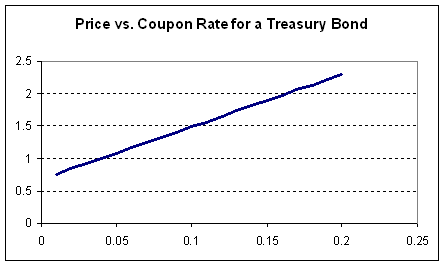
\includegraphics[scale=0.7]{regbond.png}\\
\end{center}
The following graph shows the price versus coupon rate for an MBS generated by our model. Immediately we notice that it has a negative convexity. This negative convexity is due the prepayment property of MBS. Up to a certain point, the MBS acts like a Treasury bond. However, once the coupon rate (and hence the correponding mortgage rate) becomes higher, the borrowers have more incentive and opportunity to refinance. The refinancing causes prepayments, making the bond less valuable than it would otherwise be.
\begin{center}
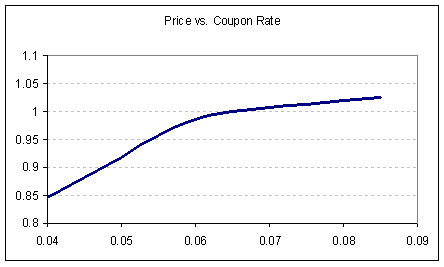
\includegraphics[scale=0.7]{negconvexity.png}\\
\end{center}
\subsection{Hedging}
Now that we have derived a price for MBS from our model, the question remains as to how to hedge our position in MBS.
\subsubsection{First approach - Duration and Convexity Hedging}
Unfortunately, this is an unusually difficult endeavour. Even a simple strategy involving duration and convexity hedging faces the problem of an appropriate definition of duration and convexity\footnote{see Fabozzi 2004 for discussion}.  However, if we follow the current convention of OAS duration and convexity, hedging becomes a matter of holding the portfolio $P + q_1 H_1 + q_2 H_2$ where $P$ is the position in MBS, $H_i$ is the price of a hedging instrument and $q_i$ is the quantity of the hedging instrument. We solve for $q_i$ using:
\begin{eqnarray}
P' + q_1 (H_1)' + q_2 (H_2)' = 0\\
P'' + q_1 (H_1)'' + q_2 (H_2)'' = 0
\end{eqnarray}
Where $P'$ refers to the derivative of the price of MBS with respect to yield, i.e. duration, and $P''$ refers to convexity. Typical hedging instruments are Treasury note futures, interest-rate swaps and swaptions, as well as MBS with different coupon rates.
\subsubsection{Second Approach - Regression-Based Hedging}
A solution to the problem of model-dependency is an ``empirical" hedging strategy, where the hedge ratio is estimated from a simple regression:
\begin{eqnarray}
\Delta S_t = \alpha + \beta \Delta F_t + \epsilon_t \\
\end{eqnarray}
Where $\Delta$ is the first-difference operation, $S_t$ is the price (or the logarithm of the price) of MBS at time $t$, $F_t$ is the price (or logarithm) of the hedging instrument at $t$, $\epsilon_t$ is the i.i.d. random error process. The hedge ratio is then the estimated $\beta$.
\subsubsection{Third approach - Incorporating the dynamic link between MBS and Treasurys}
More recently, Bhattacharya, Sekhar and Fabozzi (2006; BSF hereafter) suggest that hedging strategies should take into account the dynamic link between the MBS and treasury markets. For instance, they posit that the hedging activity of MBS investors in the swap and treasury markets increases the volatility of interest rates, which in turn leads to higher hedging requirements by holders of large MBS portfolios. Given the size of the MBS market, they quote the popular adage that the ``mortgage tail is wagging the Treasury dog," suggesting that the dynamic link is indeed an important factor.\\
\\
BSF use a cointegration model to capture the co-dependence between MBS and treasurys in terms of a long-run equilibrium relationship in their prices. Additionally, observing that volatility in the two markets is persistent, they model volatility as a GARCH process. \\
They pick five securities to include in their cointegration model, and their long run relationship is given as:
\begin{eqnarray}
P_t^{t-note} = \lambda_0 + \lambda_1 P_t^{tba5.5} + \lambda_2 P_t^{tba6.0} + \lambda_3 P_t^{tba6.5} + \lambda_4 P_t^{tba7.0} + Corr_t
\end{eqnarray}
The corresponding error correction model for the log prices of the five securities is:
\begin{equation}
\label{fivesecurities} \Delta P_t^X = \alpha_t^X + \beta_t^X(Corr_{t-1}) + \gamma_t^X(M var_{t-1}) + \varepsilon_t^X
\end{equation}
Where $X$ takes the values $\left\lbrace tba5.5, tba6.0, tba6.5, tba7.0, t-note \right\rbrace $ and the error terms of equation $\ref{fivesecurities}$ are assumed to follow a multivariate normal distribution, and are given by $\varepsilon_t = [ \varepsilon_t^{X_1} \cdots \varepsilon_t^{X_n} ]$, with the GARCH structure given by 
\begin{eqnarray}
H_t = A'A + B'\varepsilon_{t-1}\varepsilon_{t-1}'B + C'H_{t-1}C
\end{eqnarray}
where $H_t$ is the variance-covariance matrix for the variance equations of the GARCH processes for the five securities at time $t$, $A$ is the diagonal matrix of intercepts and $B$ and $C$ are the diagonal matrices of slope coefficients of the variance equations. Hedge ratios are calculated by 
\begin{eqnarray}
w_{tba6.0} = - \dfrac{\sigma_{tba5.5, tba6.0}}{\sigma^2_{tba5.5}}
\end{eqnarray}
where $\sigma_{tba5.5,tba6.0}$ and $\sigma_{tba5.5}^2$ are part of the variance-covariance matrix generated by the model. The principal improvement of the BSF cointegration GARCH model is that it reflects two market realities - that the causal relationship between MBS and treasury prices is two-way, and that volatility is not constant across time - that the simple regression model does not.
\section{Implementation}
\begin{center}
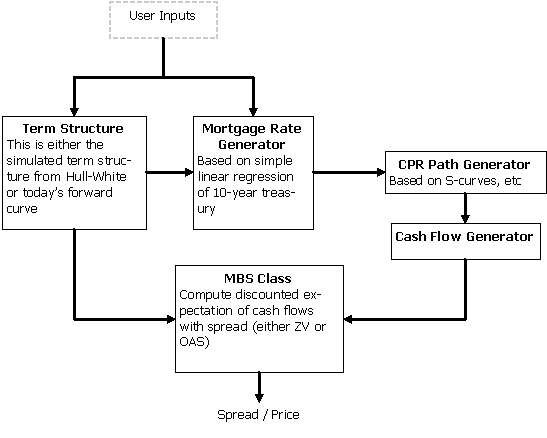
\includegraphics[scale=0.7]{classes.png}\\
\end{center}
We employ inheritance in the following manner so that we can compute either the Zero Volatility Spread or the Option Adjusted Spread without altering too much code.
\begin{center}
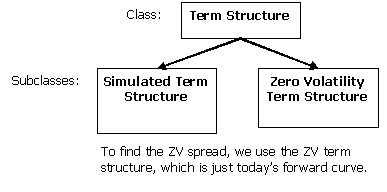
\includegraphics[scale=0.7]{inheritance.png}
\end{center}
\section{Possible Extensions to Current Implementation}
There have been several papers suggesting that house prices are a significant factor in determining prepayment rates. For instance, declines in house prices reduce mortgagors' credit quality, making it harder for them to refinance or take out new loans, thus reducing the likelihood of them moving and prepaying their existing loan (Downing, Stanton and Wallace 2005). On the other hand, rising house prices may encourage mortgagors to refinance - taking advantage of their more valuable collateral to increase the size of their loan (Lee and Pace 2006). Some papers have thus sought to model
\begin{eqnarray}
HI(t) = (H_t - H_0)
\end{eqnarray}
where $HI$ is the incentive, $H_t$ is the current regional house price and $H_0$ is the regional house price at the start of mortgage) as another factor in prepayment.\\
\\
In general, incorporating pool-specific information augments the precision of the prepayment model. Details such as average credit quality, possibly proxied by median income, are often incorporated in prepayment models.  Where a large number of factors are included, dimension-reduction techniques (e.g. PCA) are employed.
\section{Conclusion}
After programming the various components of the MBS pricing model in C++ we were able to generate reasonable ZV and OAS values. We also satisfy the basic check of negative convexity. Furthermote, we have ensured that our pricing tool exhibits sound fundamentals - a short rate model calibrated to market swap and swaption prices, and a prepayment model that is supported by both theory and historical data. Finally, we discussed several extensions to our simple implementation in terms of short rate modeling, prepayment modeling, and hedging. These are possible areas for future improvement.
\newpage
\section*{References and Data Sources}
\subsection{References}
John D. Naud, "Valuation and Hedging of Mortgage Backed Securities." April 18, 2007\\
Jian Chen, "Simulation-Based Pricing of Mortgage Backed Securities." 2004 \begin{verbatim}http://ieeexplore.ieee.org/iel5/9441/29990/01371503.pdf?tp=&isnumber=&arnumber=1371503\end{verbatim}
Justin London, \textit{Modeling derivatives in C++}. 2005\\
John Hull, Alan White. "Pricing Interest-Rate-Derivative Securities." 1990\\
Takeaki Kariya, Masaaki Kobayashi. "Pricing Mortgage-Backed Securities (MBS)." 2000\\
Andrew Kalotay, Deane Yang, Frank J. Fabozzi. "An Option-Theoretic Prepayment Model for Mortgages and Mortgage-Backed Securities." 2004\\
Min-Long Lee, R. Kelley Pace. "Local housing prices and mortgage refinancing in US cities." 2006\\
Chris Downing, Richard Stanton, Nancy Wallace. "An Empirical Test of a Two-Factor Mortgage Valuation Model: How Much do House Prices Matter?" 2005\\

\subsection{Data Sources}
Mortgage Rates: \begin{verbatim}http://www.federalreserve.gov/releases/h15/data/Weekly_Friday_/H15_MORTG_NA.txt \end{verbatim}
Treasury Yields: \begin{verbatim} http://www.ustreas.gov/offices/domestic-finance/
debt-management/interest-rate/yield_historical_huge.shtml \end{verbatim}
\newpage
\section*{Appendix: S-Plus Code for Historical Estimation}
\begin{verbatim}
#a
dt<-1/52
onemotime<-matrix(1,1160,1)
for(i in 1:1160){
	onemotime[i] = threemo[i,2]
}
onemodp<-onemotime/100		#change to decimal points from percentage
alpha<-mean(onemodp)
alphavect<-matrix(alpha,1159,1)

rtvect<-onemodp[2:1160]
rt1vect<-onemodp[1:1159]
rhonumerator<-sum((rtvect-alphavect)*(rt1vect-alphavect))
rhodenominator<-sum((rt1vect-alphavect)^2)
rho<-rhonumerator/rhodenominator

rthat<-(1-rho)*alphavect + rho*rt1vect
et<-rtvect - rthat
sigdel<-sum(et^2)/length(et)

kappa<-(-log(rho)/dt)
sig<-sqrt(2*kappa*sigdel/(1-exp(-2*kappa*dt)))
\end{verbatim}
\end{document}